\documentclass[tikz,border=7mm]{standalone}
\usepackage[T1]{fontenc}
\usepackage{xcolor}
\usepackage{amsmath,amssymb}
\usepackage{tikz}
\usetikzlibrary{positioning,arrows.meta,calc,fit,backgrounds,shapes.geometric}

\tikzset{
  flow/.style={-{Stealth[length=2.5mm]}, line width=0.9pt, draw=black!68},
  feedback/.style={-{Stealth[length=2.5mm]}, line width=0.9pt,
    dashed, draw=red!72!black},
  block/.style={draw=black!55, fill=white, rounded corners=3pt,
    minimum height=1.35cm, text width=2.05cm, align=center,
    inner xsep=4pt, font=\small},
  encoder/.style={trapezium, trapezium left angle=82, trapezium right angle=98,
    draw=blue!62!black, fill=blue!9, minimum height=1.55cm,
    text width=1.70cm, align=center, font=\small},
  decoder/.style={trapezium, trapezium left angle=98, trapezium right angle=82,
    draw=green!55!black, fill=green!9, minimum height=1.55cm,
    text width=1.70cm, align=center, font=\small},
  latent/.style={circle, draw=blue!65!black, fill=blue!14,
    minimum size=0.82cm, inner sep=0pt, font=\small},
  peakbox/.style={draw=purple!68!black, fill=purple!8, rounded corners=3pt,
    minimum height=1.05cm, text width=2.15cm, align=center, font=\small},
  outbox/.style={draw=orange!78!black, fill=orange!12, rounded corners=3pt,
    minimum height=1.05cm, text width=1.75cm, align=center, font=\small},
  badge/.style={draw=black!35, fill=black!4, rounded corners=6pt,
    inner xsep=6pt, inner ysep=3pt, font=\scriptsize},
  title/.style={font=\Large\bfseries, anchor=west},
  subtitle/.style={font=\small, text=black!58, anchor=west},
  label/.style={font=\scriptsize, text=black!60, align=center}
}


\begin{document}
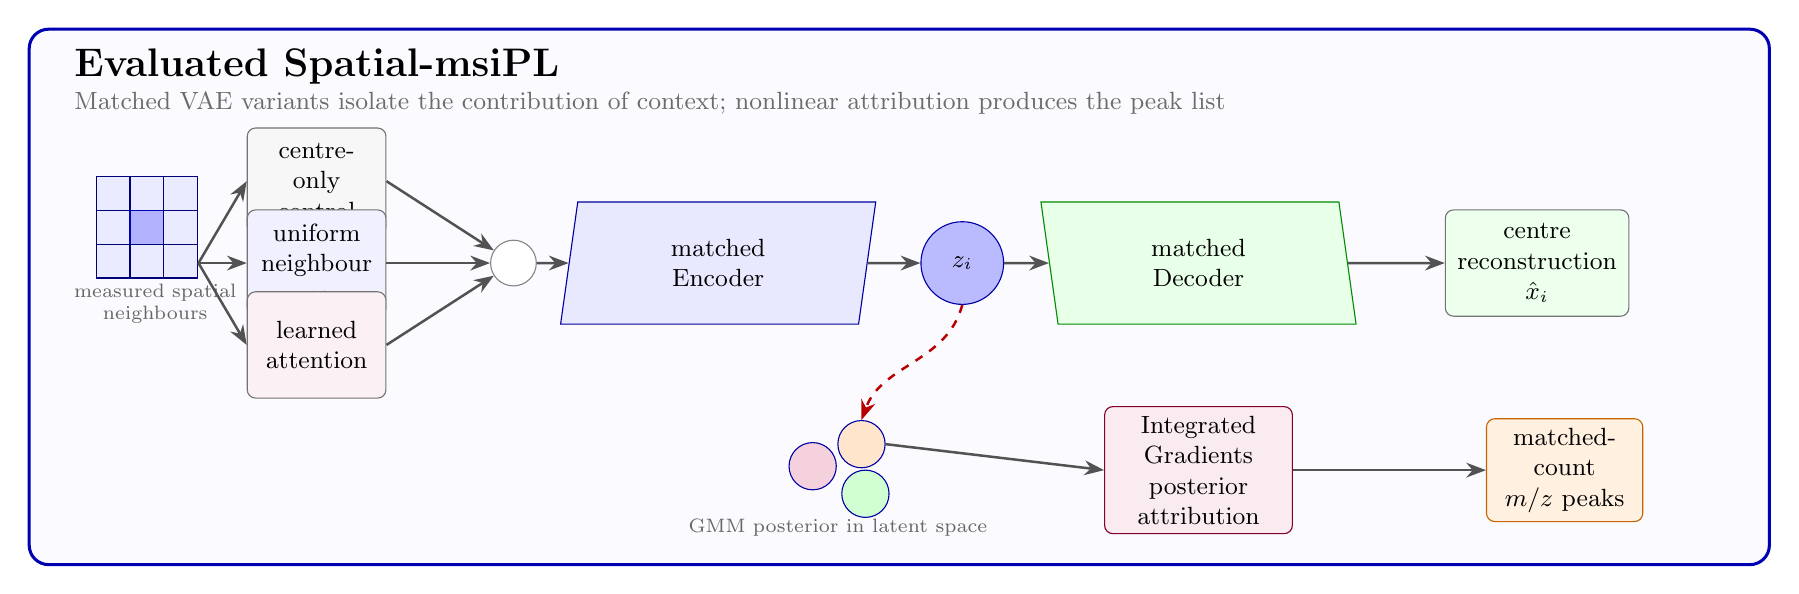
\begin{tikzpicture}[font=\sffamily]
  \fill[blue!2, rounded corners=7pt] (-0.6,2.55) rectangle (21.50,-4.25);
  \draw[blue!70!black, rounded corners=7pt, line width=1.1pt]
    (-0.6,2.55) rectangle (21.50,-4.25);
  \node[title] at (-0.15,2.08) {Evaluated Spatial-msiPL};
  \node[subtitle] at (-0.15,1.61)
    {Matched VAE variants isolate the contribution of context; nonlinear attribution produces the peak list};

  % Measured neighbourhood.
  \foreach \r in {0,1,2}{
    \foreach \c in {0,1,2}{
      \pgfmathtruncatemacro{\iscenter}{(\r==1 && \c==1)}
      \ifnum\iscenter=1
        \filldraw[draw=blue!72!black, fill=blue!30]
          ($(0.25,0.68)+(0.43*\c,-0.43*\r)$) rectangle ++(0.43,-0.43);
      \else
        \filldraw[draw=blue!48!black, fill=blue!8]
          ($(0.25,0.68)+(0.43*\c,-0.43*\r)$) rectangle ++(0.43,-0.43);
      \fi
    }
  }
  \node[label, text width=2.35cm] at (1.00,-0.94) {measured spatial neighbours};

  \node[block, fill=black!3, text width=1.48cm] (central) at (3.05,0.62)
    {centre-only\\control};
  \node[block, fill=blue!6, text width=1.48cm] (uniform) at (3.05,-0.42)
    {uniform\\neighbour mean};
  \node[block, fill=purple!6, text width=1.48cm] (attention) at (3.05,-1.46)
    {learned\\attention};
  \node[circle, draw=black!48, fill=white, minimum size=0.58cm,
    inner sep=0pt] (merge) at (5.55,-0.42) {};
  \node[encoder] (enc) at (8.15,-0.42) {matched\\Encoder};
  \node[latent, fill=blue!27, minimum size=1.05cm] (z) at (11.25,-0.42) {$z_i$};
  \node[decoder] (dec) at (14.25,-0.42) {matched\\Decoder};
  \node[block, fill=green!7] (recon) at (18.55,-0.42)
    {centre\\reconstruction $\hat{x}_i$};

  \draw[flow] (1.55,-0.42) -- (central.west);
  \draw[flow] (1.55,-0.42) -- (uniform.west);
  \draw[flow] (1.55,-0.42) -- (attention.west);
  \draw[flow] (central.east) -- (merge);
  \draw[flow] (uniform.east) -- (merge);
  \draw[flow] (attention.east) -- (merge);
  \draw[flow] (merge.east) -- (enc.west);
  \draw[flow] (enc.east) -- (z.west);
  \draw[flow] (z.east) -- (dec.west);
  \draw[flow] (dec.east) -- (recon.west);

  \node[latent, minimum size=0.60cm, fill=purple!18] (g1) at (9.35,-3.00) {};
  \node[latent, minimum size=0.60cm, fill=orange!20] (g2) at (9.97,-2.72) {};
  \node[latent, minimum size=0.60cm, fill=green!18] (g3) at (10.02,-3.35) {};
  \node[label] at (9.67,-3.78) {GMM posterior in latent space};
  \node[peakbox] (ig) at (14.25,-3.05)
    {Integrated Gradients\\posterior attribution};
  \node[outbox] (peaks) at (18.90,-3.05)
    {matched-count\\$m/z$ peaks};
  \draw[feedback] (z.south) to[out=-105,in=70] (g2.north);
  \draw[flow] (g2.east) -- (ig.west);
  \draw[flow] (ig) -- (peaks);
\end{tikzpicture}
\end{document}
